\documentclass[index]{GeM-UPM}

\usepackage{float}


%%%%%%%%%%%%%%%%%%%%%%%%%%%%%%%%%%%%%%%%%%%%%%%%%%%%%%%%%%%%%%%%%%%%%%%%
% TITULO, AUTORES Y DIRECTORES
%
\title{QuadFix: \\ Rectificador de Imágenes}
\author{Carmen Toribio, Marcos Carnerero, María Moronta}
\genderauthor{M}
\bibauthor {Toribio, Carmen,  Carnerero, Marcos,  Moronta, María}
\tutor{Jonatan Sanchez}
\bibtutor{Sanchez, Jonatan}
\fecha{9 de junio de 2025}

%%%%%%%%%%%%%%%%%%%%%%%%%%%%%%%%%%%%%%%%%%%%%%%%%%%%%%%%%%%%%%%%%%%%%%%%%%%%%%%%
% ENTORNOS MATEMÁTICOS
%
\newtheoremstyle{theoremGeM}% name of the style to be used
  {\topsep}% measure of space to leave above the theorem. E.g.: 3pt
  {\topsep}% measure of space to leave below the theorem. E.g.: 3pt
  {\itshape}% name of font to use in the body of the theorem
  {0pt}% measure of space to indent
  {\bfseries\color{schoolcolor}}% name of head font
  {.}% punctuation between head and body
  { }% space after theorem head; " " = normal interword space
  {\thmname{#1}\thmnumber{ #2}\textnormal{\thmnote{ (#3)}}}

% Nuevos teoremas
\theoremstyle{theoremGeM}
\newtheorem{thm}{Teorema}[chapter]
\newtheorem{prop}[thm]{Proposición}
\newtheorem{lem}[thm]{Lema}

% Cambiamos el color de la demostración
\AtBeginDocument{\renewcommand*{\proofname}{\color{schoolcolor}Demostración}}

\newtheoremstyle{remarkGeM}% name of the style to be used
  {\topsep}% measure of space to leave above the theorem. E.g.: 3pt
  {\topsep}% measure of space to leave below the theorem. E.g.: 3pt
  {}% name of font to use in the body of the theorem
  {0pt}% measure of space to indent
  {\itshape\color{schoolcolor}}% name of head font
  {.}% punctuation between head and body
  { }% space after theorem head; " " = normal interword space
  {\thmname{#1}\thmnumber{ #2}\textnormal{\thmnote{ (#3)}}}

\theoremstyle{remarkGeM}
\newtheorem*{rmk}{Observación}
\newtheorem{exm}[thm]{Ejemplo}

\newtheoremstyle{definitionGeM}% name of the style to be used
  {\topsep}% measure of space to leave above the theorem. E.g.: 3pt
  {\topsep}% measure of space to leave below the theorem. E.g.: 3pt
  {}% name of font to use in the body of the theorem
  {0pt}% measure of space to indent
  {\bfseries\color{schoolcolor}}% name of head font
  {.}% punctuation between head and body
  { }% space after theorem head; " " = normal interword space
  {\thmname{#1}\thmnumber{ #2}\textnormal{\thmnote{ (#3)}}}
\theoremstyle{definitionGeM}
\newtheorem{defn}[thm]{Definition}

%%%%%%%%%%%%%%%%%%%%%%%%%%%%%%%%%%%%%%%%%%%%%%%%%%%%%%%%%%%%%%%%%%%%%%%%
% DOCUMENTO
%

\begin{document}

% !TEX root = ../main.tex

\chapter{Introducción}
\label{ch:introduccion}
Hoy en día, es muy común usar dispositivos móviles para tomar fotos de \textbf{objetos planos}, como folios, pizarras o carteles. Sin embargo, estas imágenes suelen tener \textbf{distorsiones} por el ángulo desde el que se toman, lo que hace que un documento se vea como una figura irregular. Este proyecto soluciona ese problema utilizando una técnica llamada \textbf{rectificación proyectiva}, que permite recuperar la \textbf{forma original} de esos objetos planos.

Para solucionar este problema, desarrollamos una herramienta llamada \textbf{QuadFix}, que combina conceptos de \textbf{geometría proyectiva} con un enfoque interactivo. El usuario simplemente selecciona las \textbf{cuatro esquinas} del objeto en la imagen y el sistema aplica una transformación llamada \textbf{homografía} para generar una nueva imagen con una vista frontal, manteniendo las \textbf{proporciones} del objeto. 

Para crear esta herramienta usamos \textbf{Python} y algunas librerías importantes. \textbf{NumPy} nos ayudó a hacer cálculos matriciales de manera eficiente, lo que fue clave para resolver el sistema de ecuaciones que permite la transformación. Por otro lado, \textbf{PySide6 (Qt)} nos permitió construir una \textbf{interfaz gráfica} sencilla y fácil de usar, que incluye funciones como la selección de puntos, el ajuste de proporciones y la \textbf{visualización en tiempo real} de los cambios.

El desarrollo se dividió en tres partes principales. Primero, implementamos la \textbf{rectificación básica}, que corrige cualquier cuadrilátero irregular y lo transforma en un cuadrado usando homografías. Luego, extendimos el sistema para manejar \textbf{proporciones específicas}, como los rectángulos con una relación de aspecto particular, por ejemplo el formato \textbf{DIN A4}, que tiene una proporción aproximada de \(\sqrt{2}:1\). Por último, diseñamos una \textbf{interfaz} que acompaña al usuario durante todo el proceso, desde cargar la imagen hasta guardar el resultado.

A lo largo de este documento se describen con detalle los \textbf{fundamentos teóricos} que sustentan la rectificación proyectiva, el \textbf{desarrollo técnico} dividido en sus distintas fases, y se presentan \textbf{ejemplos prácticos} que ilustran la funcionalidad y utilidad de la herramienta.


% !TEX root = ../main.tex

\chapter{Fundamentos Teóricos}
\label{ch:fundamentos}

El presente capítulo establece los \textbf{fundamentos teóricos} sobre los cuales se construye el desarrollo del sistema de \textbf{rectificación de imágenes} propuesto. Para comprender el funcionamiento y las decisiones de diseño adoptadas, es imprescindible revisar conceptos clave de la \textbf{geometría proyectiva}, las \textbf{homografías} y las \textbf{transformaciones métricas}. Estas herramientas matemáticas permiten modelar y revertir las deformaciones por perspectiva que se producen en fotografías de objetos planos, facilitando así su representación frontal sin distorsiones. A través de este marco teórico se justifica tanto la \textbf{viabilidad del proceso de rectificación} como las \textbf{simplificaciones prácticas} implementadas en el sistema, que buscan un equilibrio entre rigor matemático, facilidad de uso y eficiencia computacional.


\section{Rectificación de Imágenes}

La \textbf{rectificación proyectiva} es el proceso mediante el cual se elimina la distorsión causada por la perspectiva en una imagen, con el fin de obtener una representación frontal y sin deformaciones de un objeto plano. Este proceso es fundamental cuando se trabaja con imágenes tomadas desde ángulos no perpendiculares, como ocurre frecuentemente al fotografiar documentos, pizarras o carteles con dispositivos móviles.

Desde un punto de vista teórico, una imagen tomada con una cámara convencional es una proyección central del mundo tridimensional sobre un plano bidimensional. Debido a esta proyección, las líneas paralelas en el mundo real pueden aparecer convergentes en la imagen (fenómeno conocido como \textit{perspectiva}), y las formas geométricas regulares se ven deformadas, transformándose en cuadriláteros irregulares.

La rectificación consiste en encontrar una transformación planar —específicamente, una homografía— que deshaga esta proyección, reconstruyendo la vista frontal del objeto plano y restaurando sus propiedades métricas, como la forma y las proporciones.

Matemáticamente, si el objeto plano en el mundo real puede representarse mediante un sistema de coordenadas en un plano, la imagen proyectada corresponde a una transformación de ese plano mediante una homografía \(H\). Si \( \mathbf{x} = (x, y, 1)^T \) es un punto en la imagen distorsionada, existe una homografía \(H\) tal que

\begin{equation}
    \mathbf{x}' = H \mathbf{x},
\end{equation}


donde \(\mathbf{x}'\) corresponde al punto en la imagen rectificada, idealmente en la posición que tendría si la cámara estuviera perpendicular al objeto. Para calcular esta homografía, se requieren al menos cuatro puntos no colineales en la imagen original y sus correspondientes puntos en la imagen deseada (normalmente, los vértices de un rectángulo que representa la forma real del objeto). Esta correspondencia permite resolver un sistema de ecuaciones lineales que determina los parámetros de \(H\), pero este tema se tratará con más detalle en el punto a continuación.

El proceso de rectificación implica entonces tres pasos fundamentales:

\begin{enumerate}
  \item \textbf{Identificación de correspondencias:} Selección de los cuatro puntos en la imagen original que delimitan el objeto plano.
  \item \textbf{Cálculo de la homografía:} Resolución del sistema lineal para encontrar la matriz \(H\) que mapea esos puntos a un rectángulo con las proporciones reales.
  \item \textbf{Aplicación de la transformación:} Uso de \(H\) para transformar toda la imagen, corrigiendo la perspectiva y generando la imagen rectificada.
\end{enumerate}

Es importante destacar que esta transformación preserva la linealidad (es decir, las líneas rectas permanecen rectas), pero no garantiza la conservación de distancias o ángulos, ya que una homografía general sólo preserva propiedades proyectivas. Sin embargo, en aplicaciones como la nuestra, donde se busca que el objeto rectificado mantenga sus \textbf{proporciones reales}, es necesario realizar ajustes adicionales para \textbf{restaurar la métrica euclidiana}. Para ello, se pueden emplear técnicas que estiman la \textit{línea del infinito} y los \textit{puntos de fuga}, permitiendo recuperar propiedades métricas del plano original.

Durante la aplicación de una transformación proyectiva, es necesario reasignar el valor de cada píxel en la imagen rectificada, ya que las coordenadas resultantes suelen ser valores reales y no enteros, que no corresponden directamente a posiciones exactas en la imagen original. Para resolver este problema se utilizan técnicas de \textbf{interpolación}, cuyo objetivo es estimar el valor del píxel en una posición no entera a partir de los valores de píxeles vecinos con coordenadas enteras.

Uno de los métodos más simples y eficientes es la \textbf{interpolación por vecino más cercano} (nearest neighbor). Este método consiste en asignar al píxel transformado el valor del píxel original que se encuentra en la posición entera más próxima a las coordenadas reales calculadas.

\label{sec:metodo_vecino}

\vspace{\baselineskip}

Por otro lado, la rectificación de imágenes es sumamente útil en múltiples aplicaciones:

\begin{itemize}
  \item \textbf{Digitalización de documentos:} Fotografías tomadas con smartphones que deforman folios o pizarras pueden corregirse para obtener imágenes limpias y planas.
  \item \textbf{Fotogrametría:} Permite reconstruir modelos 3D a partir de imágenes 2D mediante la corrección de perspectivas.
  \item \textbf{Diseño gráfico:} Facilita la corrección de perspectivas en carteles, logotipos u otros elementos visuales deformados.
\end{itemize}

En resumen, la rectificación proyectiva es una herramienta matemática y computacional esencial para convertir imágenes deformadas por perspectiva en representaciones frontales precisas, facilitando la digitalización, el análisis y la manipulación de objetos planos.


\section{Geometría Proyectiva y Homografías}

Como se mencionó anteriormente, la herramienta fundamental para la rectificación de imágenes es la \textbf{homografía}, una transformación proyectiva que proviene de la \textbf{geometría proyectiva}. Esta rama de las matemáticas estudia las propiedades de las figuras que permanecen invariantes bajo transformaciones proyectivas, como las perspectivas que vemos en fotografías.

A diferencia de la geometría euclidiana —que conserva distancias, ángulos y paralelismo—, la geometría proyectiva preserva propiedades más generales, como la \textbf{incidencia} (puntos alineados sobre una misma recta), la \textbf{colinealidad} y la \textbf{razón doble} (una proporción invariante entre cuatro puntos colineales bajo transformaciones proyectivas).

En este contexto, una \textbf{homografía} es una función que relaciona dos planos proyectivos mediante una matriz \(3 \times 3\). Esta matriz actúa sobre puntos expresados en coordenadas homogéneas, lo que permite manejar de forma compacta transformaciones que incluyen proyecciones y efectos de perspectiva.

Sea un punto en coordenadas homogéneas \(\mathbf{x} = (x, y, w)^T\) en el plano original, la homografía \(H\) produce el punto transformado:

\begin{equation}
\mathbf{x}' = H \mathbf{x} =
\begin{pmatrix}
h_{11} & h_{12} & h_{13} \\
h_{21} & h_{22} & h_{23} \\
h_{31} & h_{32} & h_{33}
\end{pmatrix}
\begin{pmatrix}
x \\ y \\ w
\end{pmatrix}
=
\begin{pmatrix}
x' \\ y' \\ w'
\end{pmatrix}.
\label{eq:homografia}
\end{equation}

Esta transformación tiene la propiedad fundamental de preservar la \textbf{linealidad}, es decir, las líneas rectas en el plano original se mapean en líneas rectas en el plano transformado. Sin embargo, no se garantiza la conservación de distancias, ángulos ni proporciones, lo que implica que la imagen resultante puede estar deformada desde un punto de vista métrico.

\subsection*{Cálculo de la homografía}

En nuestro sistema, la matriz de homografía \(H\) se calcula directamente a partir de información geométrica obtenida de la imagen, mediante un proceso basado en álgebra lineal. El procedimiento consta de los siguientes pasos principales:

\begin{enumerate}
    \item \textbf{Selección de puntos de entrada:} El usuario proporciona cuatro puntos no colineales que definen el contorno del objeto plano a rectificar (por ejemplo, los vértices de un folio o cartel en una imagen tomada en perspectiva).

    \item \textbf{Cálculo de puntos de fuga:} Se construyen las rectas que corresponden a los lados opuestos del cuadrilátero, y se obtienen sus intersecciones en coordenadas homogéneas. Estas intersecciones definen los \textit{puntos de fuga} \(\mathbf{v}_1\) y \(\mathbf{v}_2\), que caracterizan la dirección de las líneas paralelas en el espacio original:
    \[
    \ell_1 = \mathbf{x}_1 \times \mathbf{x}_2, \quad \ell_2 = \mathbf{x}_3 \times \mathbf{x}_4, \quad \Rightarrow \quad \mathbf{v}_1 = \ell_1 \times \ell_2,
    \]
    \[
    \ell_3 = \mathbf{x}_2 \times \mathbf{x}_3, \quad \ell_4 = \mathbf{x}_4 \times \mathbf{x}_1, \quad \Rightarrow \quad \mathbf{v}_2 = \ell_3 \times \ell_4.
    \]
    Aquí, \(\times\) denota el producto cruzado en coordenadas homogéneas.

    \item \textbf{Construcción del sistema lineal:} Se plantea un sistema de ecuaciones para determinar los coeficientes de la matriz \(H\), tal que:
    \begin{itemize}
        \item \(\mathbf{v}_1\) y \(\mathbf{v}_2\) se transformen en las direcciones canónicas \([1,0,0]^T\) y \([0,1,0]^T\).
        \item Dos vértices opuestos del cuadrilátero (que serían \(\mathbf{x}_1\) y \(\mathbf{x}_4\) en nuestro caso) se fijen en coordenadas específicas del plano destino, lo cual establece la escala y orientación de la imagen rectificada.
    \end{itemize}
    La resolución de este sistema proporciona directamente la matriz de homografía \(H\).

    \item \textbf{Ajuste de razón de aspecto:} Para garantizar que la imagen rectificada refleje fielmente las proporciones reales del objeto (por ejemplo, un folio DIN A4 o un cartel cuadrado), se aplica una transformación de escala anisotrópica mediante la siguiente matriz:
    \[
    S = 
    \begin{pmatrix}
    b & 0 & 0 \\
    0 & c & 0 \\
    0 & 0 & 1
    \end{pmatrix},
    \]
    donde los factores \(b\) y \(c\) se escogen de forma que la razón \(c/b\) coincida con la razón de aspecto deseada (proporción altura/ancho). La homografía final se obtiene entonces como:
    \[
    H' = S \cdot H.
    \]
\end{enumerate}

Este enfoque directo resulta más eficiente y fácil de controlar en la práctica, ya que permite obtener una transformación completa sin descomponerla en pasos intermedios. Refleja fielmente la implementación del sistema y proporciona una base sólida para una rectificación proyectiva robusta.



\section{Preservación Métrica y Razón de Aspecto}

Aunque una homografía general garantiza la preservación de propiedades proyectivas como la colinealidad y la incidencia, no conserva en general la métrica euclidiana, es decir, las distancias y ángulos reales. Sin embargo, en muchas aplicaciones prácticas (entre ellas, la nuestra), es fundamental que la imagen rectificada mantenga las proporciones del objeto.

Para ello, es necesario considerar conceptos como los \textbf{puntos de fuga}, también conocidos como puntos en el infinito, y la \textbf{línea del infinito} en el plano proyectivo. Las líneas paralelas en el mundo real convergen en puntos de fuga en la imagen, debido a la perspectiva. Su identificación permite localizar la línea del infinito, fundamental para restaurar propiedades métricas como los ángulos rectos y las proporciones reales.

En teoría, si se conoce la línea del infinito, se puede aplicar una transformación adicional denominada \textbf{homografía métrica} que recupera la métrica euclidiana. Sin embargo, dado que en nuestro proyecto el usuario define manualmente las cuatro esquinas del objeto, adoptamos un enfoque práctico basado en la especificación directa de la razón de aspecto deseada. El usuario introduce la proporción altura/ancho (\textit{aspect ratio}) real del objeto, por ejemplo:

\begin{itemize}
    \item Cuadrado: \(1:1\)
    \item Folio DIN A4 (vertical): \(\approx \sqrt{2}:1 \approx 1.4142:1\)
\end{itemize}

Esta razón se incorpora en la homografía final mediante una \textbf{homotecia}, que es una transformación afín que realiza un escalado diferencial en las direcciones del plano, ajustando así las dimensiones de la imagen rectificada para que cumpla con la proporción deseada. Matemáticamente, esta homotecia se representa mediante la matriz de escala diagonal que se encuentra a continuación

\[
S = 
\begin{pmatrix}
b & 0 & 0 \\
0 & c & 0 \\
0 & 0 & 1
\end{pmatrix},
\]

donde los factores \(b\) y \(c\) se eligen para que la razón \(b/c\) coincida con la proporción especificada. Por ejemplo, si \(r = \text{alto}/\text{ancho}\) es la razón deseada, se puede tomar \(b=1\) y \(c=r\) (o viceversa según normalización).

Otro concepto relevante dentro de la geometría proyectiva es la \textbf{razón doble}, un \textit{invariante proyectivo} que se mantiene constante bajo transformaciones proyectivas y que, en teoría, puede utilizarse para recuperar información métrica (como proporciones o distancias relativas) sin necesidad de conocer previamente las dimensiones reales del objeto. No obstante, en este proyecto hemos decidido no emplearla por varias razones:

\begin{itemize}
    \item \textbf{Simplicidad y usabilidad:} Incluir el cálculo de la razón doble implicaría pedir al usuario que identifique puntos adicionales con precisión (por ejemplo, cuatro puntos colineales con una distribución significativa), lo cual complicaría considerablemente tanto la interfaz como la experiencia de uso. Nuestro enfoque busca minimizar la intervención técnica por parte del usuario.
    
    \item \textbf{Precisión práctica:} En la mayoría de los casos de uso contemplados, como la rectificación de documentos, el usuario ya conoce la \textbf{razón de aspecto} del objeto (pues están escritas las proporciones más básicas en un apartado de la interfaz de usuario llamado ``Instrucciones''). Esta proporción es más intuitiva, fácil de introducir y menos propensa a errores que intentar estimar una razón doble sobre una imagen deformada.
    
    \item \textbf{Eficiencia computacional:} La estimación de la razón doble requiere identificar características adicionales (como líneas paralelas u ortogonales), lo que implicaría procesos más complejos y costosos en términos de cómputo. En cambio, aplicar una \textbf{homotecia} (un escalado uniforme o anisotrópico) sobre la imagen rectificada a partir de una razón de aspecto conocida es inmediato y computacionalmente eficiente.
\end{itemize}

Este método es robusto y fácil de usar, pues requiere solo cuatro puntos y una razón de aspecto conocida. No obstante, si la razón introducida no es correcta, la imagen puede resultar estirada o comprimida. Para minimizar este riesgo, la interfaz ofrece valores predefinidos comunes, como \textit{Cuadrado} o \textit{DIN A4}.

\vspace{\baselineskip}

En resumen, la combinación de homografías con ajustes métricos mediante homotecias ofrece un \textbf{equilibrio entre precisión y simplicidad}, permitiendo rectificar imágenes que conservan las proporciones reales del objeto con un procedimiento práctico y efectivo.
% !TEX root = ../main.tex

\chapter{Desarrollo del Proyecto}
\label{ch:otro}

El desarrollo del proyecto se llevó a cabo en tres fases bien diferenciadas, con el objetivo de construir progresivamente una herramienta robusta, funcional y orientada a la experiencia del usuario. A través de una metodología incremental, se fueron implementando las funcionalidades principales desde una primera versión básica hasta llegar a una aplicación completa y adaptativa.

\section{Fase 1: Rectificación Básica}

\textbf{Objetivo:} Implementar la funcionalidad base que permitiera rectificar imágenes de superficies cuadradas a través de transformaciones proyectivas.

\vspace{\baselineskip}

\textbf{Tareas Realizadas:}

\begin{itemize}
    \item \textbf{Creación de la ventana principal:} \\
    Se diseñó una interfaz gráfica básica utilizando la biblioteca \texttt{PySide6}, que permite combinar Python con Qt para el desarrollo de interfaces modernas. Esta ventana principal muestra la imagen cargada por el usuario y permite interactuar con ella. \\
    Para ello, se implementó la clase \texttt{ClickArea}, para gestionar la interacción con la imagen y permitir seleccionar puntos sobre ella mediante clics del ratón.
    
    \item \textbf{Captura y gestión de coordenadas:} \\
    Para estructurar y manipular las coordenadas de manera eficiente, se desarrolló la clase \texttt{Coordinates}. Esta clase encapsula toda la lógica relacionada con el almacenamiento y validación de los puntos seleccionados por el usuario. Entre sus funcionalidades principales se incluye la capacidad de \textbf{almacenar hasta cuatro puntos}, que son aquellos seleccionados mediante clics.
    
    Además, la clase permite \textbf{eliminar un punto} si el usuario hace clic nuevamente sobre él, facilitando la corrección y modificación de la selección. Finalmente, incorpora una \textbf{validación automática} que asegura que se hayan seleccionado exactamente cuatro puntos antes de proceder con la transformación, garantizando así la integridad de los datos para las operaciones posteriores.
    
    
    \item \textbf{Cálculo de los puntos de fuga:} \\
    El cálculo de los puntos de fuga se implementó en el módulo \texttt{infinity\_line.py}, en la función \texttt{calculate\_vanish\_points}. Esta función recibe como entrada cuatro puntos que definen un cuadrilátero sobre la imagen y calcula las intersecciones de los pares de lados opuestos. En concreto, se obtienen dos puntos de fuga mediante la intersección de las siguientes rectas:
    
    \begin{itemize}
        \item La recta que une los puntos $p_1$ y $p_2$ con la que une $p_3$ y $p_4$.
        \item La recta que une los puntos $p_1$ y $p_3$ con la que une $p_2$ y $p_4$.
    \end{itemize}
    
    Estas intersecciones se resuelven mediante álgebra lineal usando la regla de Cramer en \textbf{coordenadas cartesianas}, sin utilizar coordenadas homogéneas. El resultado se devuelve como puntos con $w = 1$, pero los cálculos no son proyectivos en sentido estricto.
        
    Los dos puntos de fuga obtenidos son utilizados posteriormente para definir la recta del infinito en otros módulos. Aunque no se calcula explícitamente la recta proyectiva como producto vectorial (e.g. con \texttt{np.cross(p, q)} en coordenadas homogéneas), esta operación puede incorporarse en el futuro para lograr una interpretación más rigurosa desde la geometría proyectiva.
    
    
    \item \textbf{Transformación proyectiva:} \\
    En el módulo \texttt{projective\_transform.py}, se desarrollaron dos funciones clave:

    \begin{itemize}
        \item \texttt{calculate\_homography}: Calcula la \textbf{matriz de homografía} que permite transformar un cuadrilátero irregular (producto de la perspectiva) en un cuadrado perfecto en la nueva imagen. La función utiliza una base de referencia estándar y resuelve el sistema mediante \textbf{álgebra lineal}.
        
        La homografía se calcula mapeando:
        \begin{itemize}
            \item Los \textbf{puntos de fuga}, obtenidos como intersecciones de lados opuestos del cuadrilátero, a direcciones canónicas \([1, 0, 0]\) y \([0, 1, 0]\).
            \item Dos \textbf{esquinas del cuadrilátero} (específicamente \(p_0\) y \(p_3\)) a posiciones fijas que determinan la escala y orientación del plano rectificado.
        \end{itemize}
        Finalmente, se aplica una \textbf{matriz de escala diagonal} (escalado anisotrópico) para ajustar la \textbf{razón de aspecto} del plano rectificado. Este escalado no representa una transformación afín completa, sino una modificación de la proporción entre ejes horizontal y vertical.
    
        \item \texttt{warp\_perspective\_qpixmap}: Aplica la homografía calculada a la imagen original para obtener una imagen \textbf{rectificada}. Esta función implementa la transformación inversa para cada píxel del plano destino: se aplica la \textbf{inversa de la homografía} para mapear cada píxel en la imagen de salida a su posición correspondiente en la imagen original. Este enfoque evita \textbf{huecos} o \textbf{solapamientos}, al garantizar que cada píxel destino proviene de una ubicación definida en la imagen fuente, pero resulta \textbf{computacionalmente ineficiente} en imágenes de gran tamaño.
    \end{itemize}
    
    \item \textbf{Integración y pruebas:} \\
    Una vez implementadas todas las funciones anteriores, se integraron en el flujo de trabajo principal de la aplicación. El usuario podía:
    \begin{enumerate}
        \item Cargar una imagen.
        \item Seleccionar 4 puntos sobre la imagen.
        \item Hacer clic en el botón “Rectificar”.
    \end{enumerate}
    La aplicación realizaba la transformación y mostraba la imagen corregida. Se llevaron a cabo pruebas con imágenes que contenían superficies cuadradas en distintas perspectivas, confirmando la efectividad de la transformación proyectiva.
\end{itemize}

\section{Fase 2: Adaptación a Otras Proporciones}

\textbf{Objetivo:} Generalizar la herramienta para que pueda rectificar no solo cuadrados, sino también rectángulos con proporciones específicas. Para ello, se añadió la posibilidad de que el usuario introduzca manualmente la razón de aspecto deseada a través de la interfaz gráfica, permitiendo así adaptar la rectificación a cualquier proporción que se requiera.

\vspace{\baselineskip}

\textbf{Tareas Realizadas:}

\begin{itemize}
    \item \textbf{Introducción de la razón de aspecto:} \\
    Se añadió un nuevo widget llamado \texttt{AspectRatioWidget} dentro del archivo \texttt{menu.py}, que permite al usuario introducir manualmente una razón de aspecto (alto/ancho). Esta se utiliza para adaptar la referencia proyectiva a las proporciones deseadas.
    
    \item \textbf{Ajuste de la homografía:} \\
    La función \texttt{calculate\_homography} fue extendida para admitir una razón de aspecto como parámetro adicional. Esta razón permite ajustar la base estándar, originalmente un cuadrado, para transformarla en un rectángulo con las proporciones deseadas.
    
    De este modo, se garantiza que la homografía resultante respete las proporciones especificadas por el usuario. Además, se incorpora un factor de escala que mantiene el tamaño visual coherente dentro de la imagen transformada, asegurando que la rectificación no distorsione la apariencia del resultado final.
    
    \item \textbf{Pruebas con rectángulos:} \\
    Se realizaron múltiples pruebas con diferentes proporciones. Los resultados confirmaron que la herramienta puede adaptarse a una amplia variedad de formatos manteniendo una alta precisión en la rectificación.
\end{itemize}

\section{Fase 3: Interfaz de Usuario}

\textbf{Objetivo:} Mejorar la experiencia del usuario con una interfaz más atractiva, intuitiva y coherente con las convenciones modernas de diseño.

\textbf{Tareas Realizadas:}

\begin{itemize}
    \item \textbf{Diseño de la interfaz:} \\
    Se reestructuró la ventana principal para incluir un menú lateral (\texttt{Menu} en \texttt{menu.py}). Este menú contiene:
    \begin{itemize}
        \item Título de la aplicación con su logo (que puede verse en la Figura~\ref{fg:logo}).
        \item Instrucciones de uso, en un apartado desplegable (apreciable en la Figura~\ref{fg:instructions}).
        \item Campo para introducir la razón de aspecto.
        \item Botones para cargar imagen, aplicar la transformación, borrar todos los puntos seleccionados y descargar la imagen una vez ha sido rectificada.
    \end{itemize}
    
    \begin{figure}[H]
        \centering	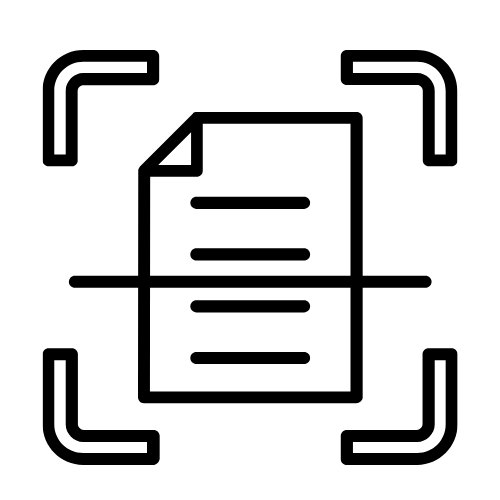
\includegraphics[width=0.2\textwidth]{figures/3.3.LogoDark.png}
        \caption{Logo de la aplicación}\label{fg:logo}
    \end{figure}
    
    \begin{figure}[H]
        \centering	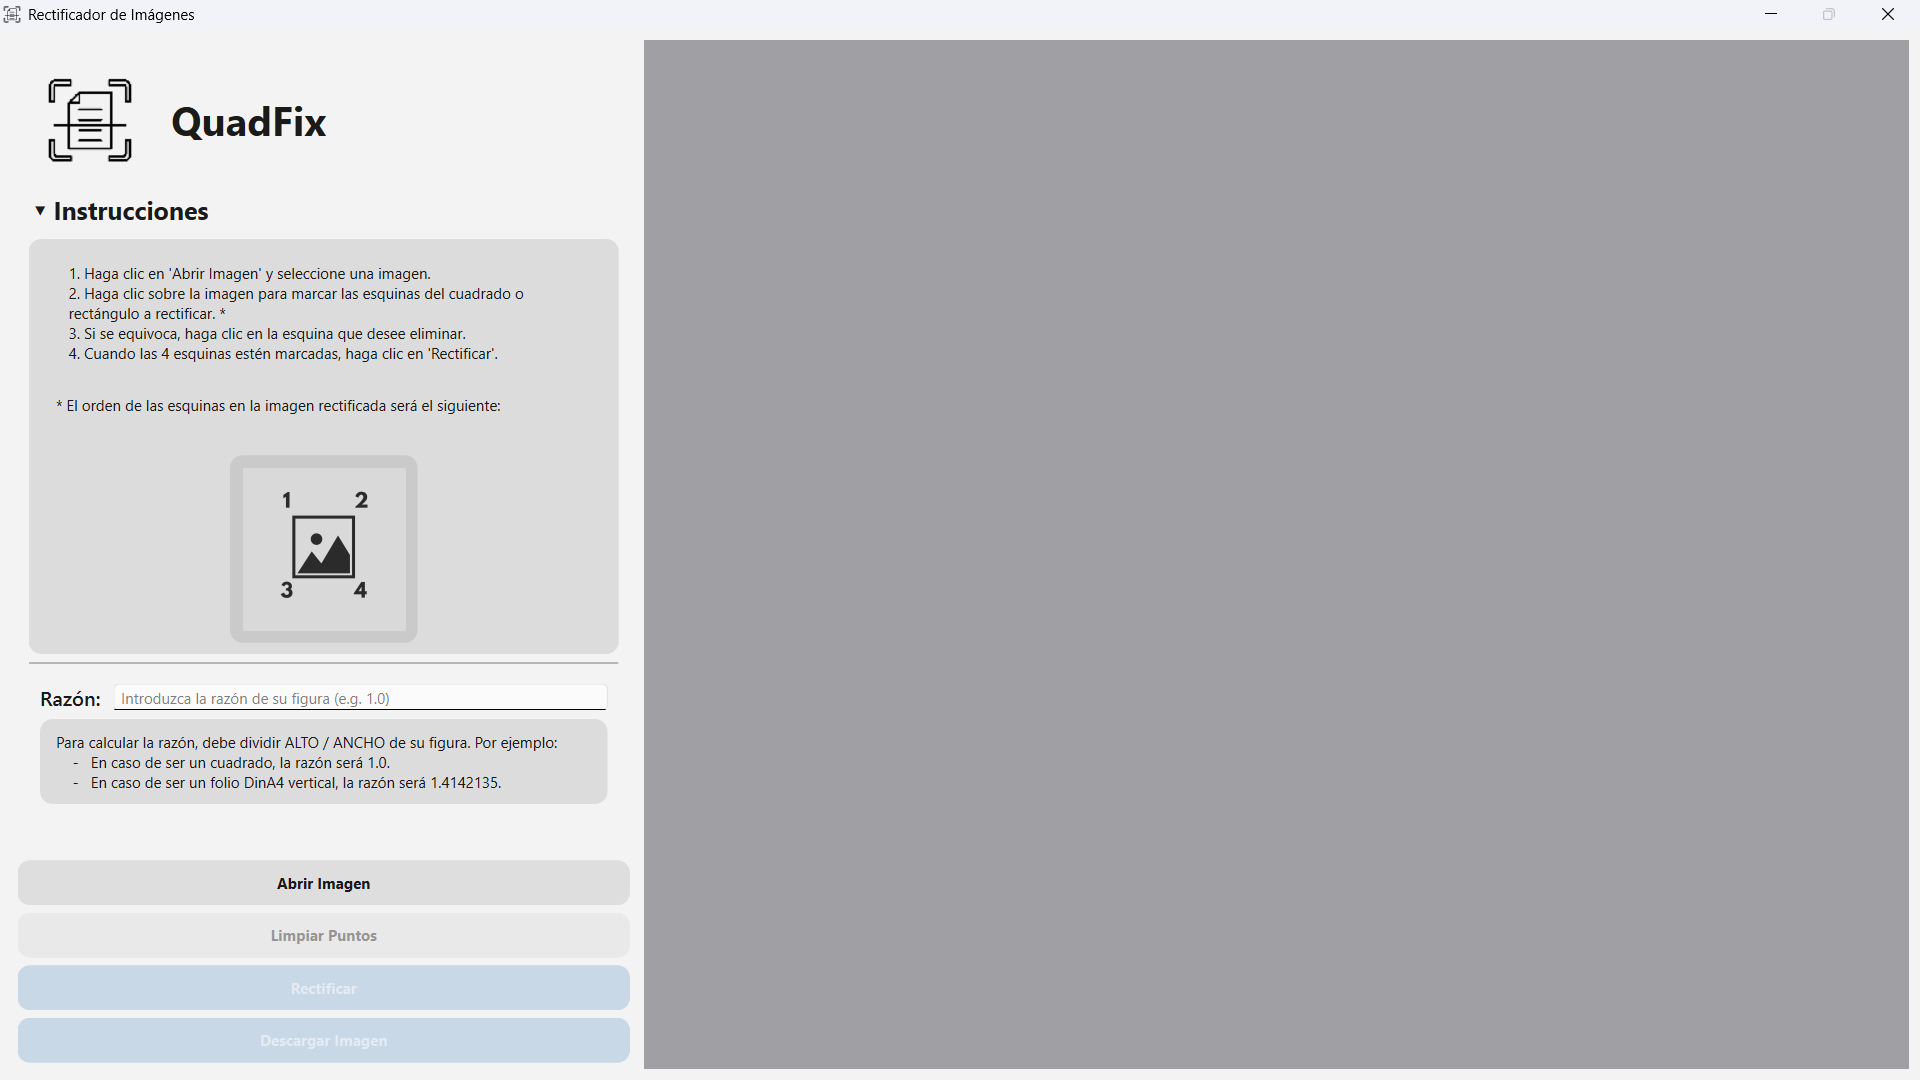
\includegraphics[width=0.8\textwidth]{figures/3.3.Instrucciones.png}
        \caption{Pantalla principal con el apartado ``Instrucciones'' desplegado}\label{fg:instructions}
    \end{figure}
    
    También se definieron dos tipos de botones personalizados, como puede apreciarse en la Figura~\ref{fg:instructions} (\texttt{PrimaryButton}, de color azul, y \texttt{SecondaryButton}, de color negro, en \texttt{buttons.py}) para mejorar la coherencia visual y la jerarquía de acciones.
    
    \item \textbf{Modo claro y oscuro:} \\
    La aplicación detecta el tema del sistema operativo mediante la función \texttt{is\_dark\_mode} (archivo \texttt{dark\_mode.py}) y adapta automáticamente los iconos, los colores del fondo, texto y contenedores y los estilos de los widgets para mantener la legibilidad. En las Figuras ~\ref{fg:light} y \ref{fg:dark} pueden verse los dos modos.

    \begin{figure}[H]
        \centering	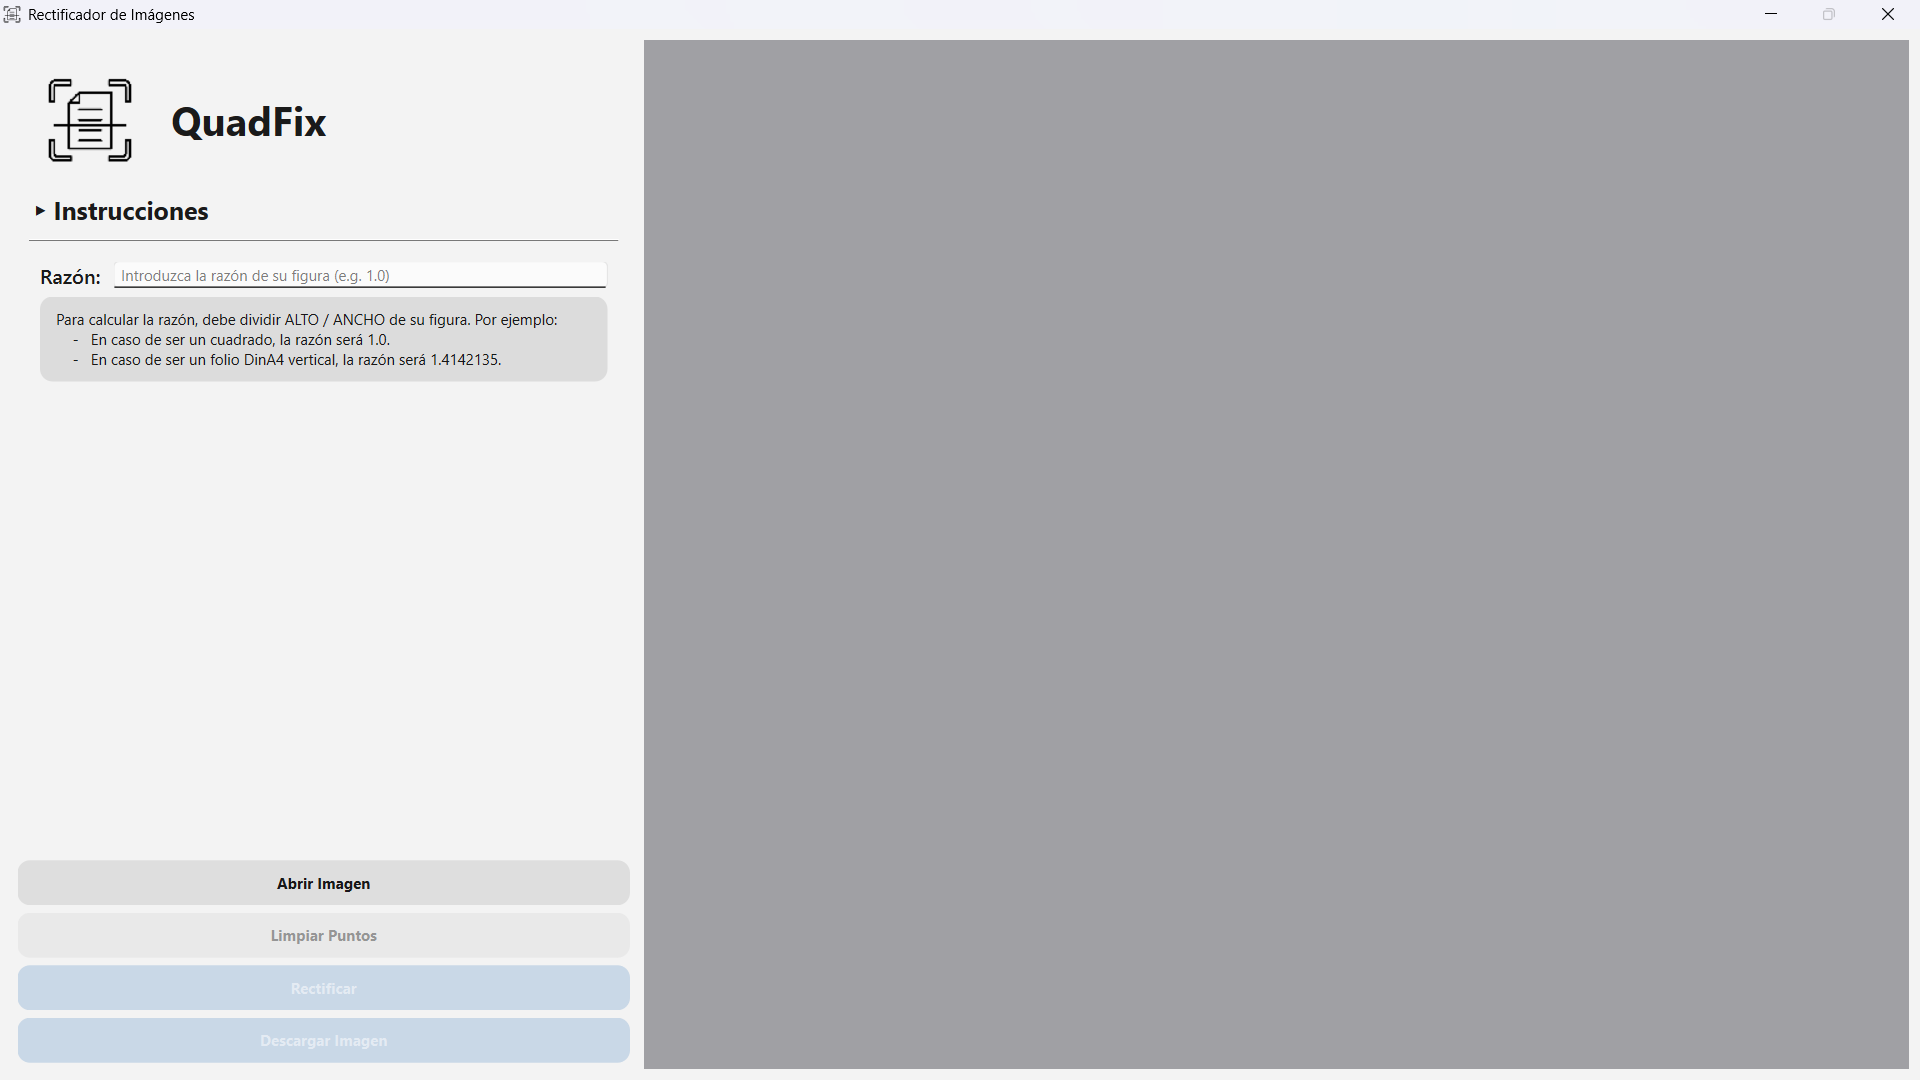
\includegraphics[width=0.65\textwidth]{figures/3.3.Light.png}
        \caption{Modo Claro de la aplicación}\label{fg:light}
    \end{figure}

    \begin{figure}[H]
        \centering	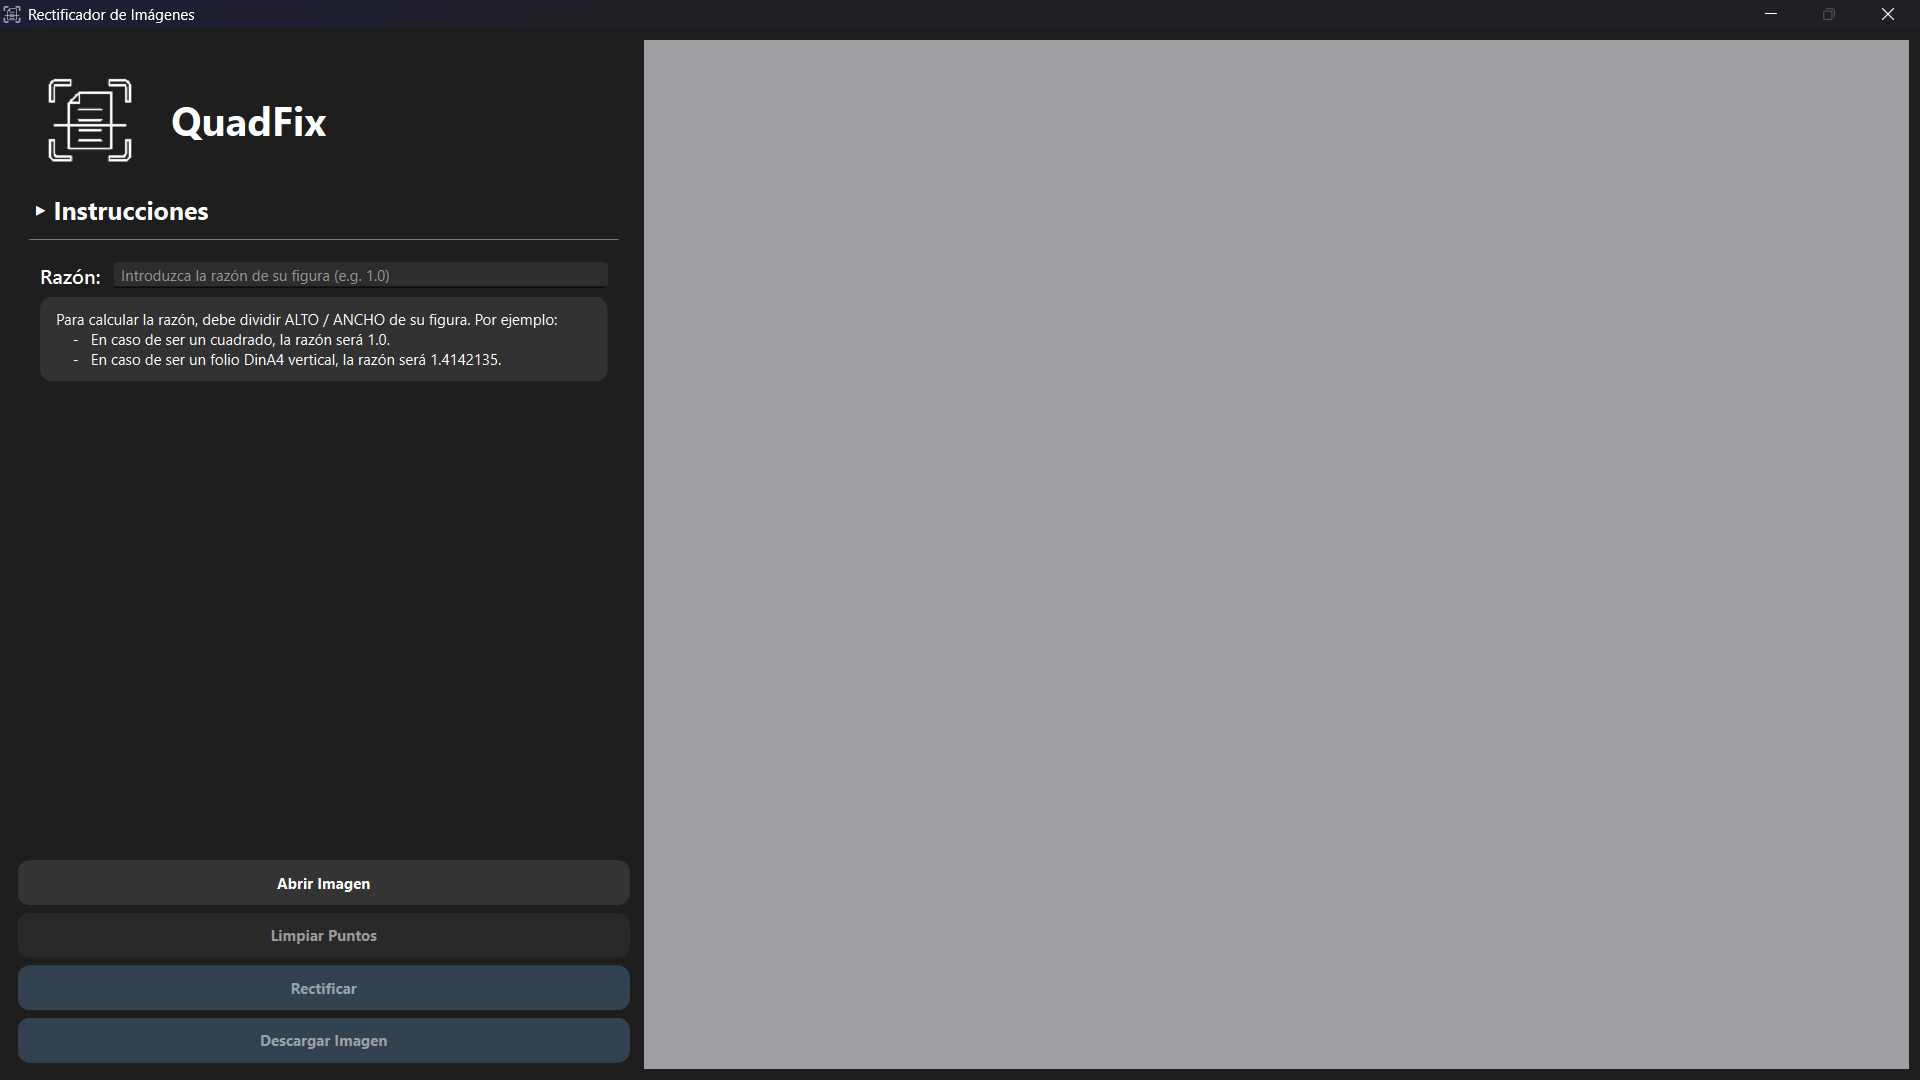
\includegraphics[width=0.65\textwidth]{figures/3.3.Dark.png}
        \caption{Modo Oscuro de la aplicación}\label{fg:dark}
    \end{figure}
    
    \item \textbf{Feedback visual al usuario:} \\
    Se incorporaron diversos mecanismos para mejorar la comunicación con el usuario durante la interacción con la aplicación. Entre estos, destaca un \textit{widget} de carga, implementado como \texttt{OverlayWidget} en el módulo \texttt{click\_area.py}, que se muestra mientras la imagen está siendo procesada.
    
    Además, se añadieron mensajes de error que alertan al usuario en caso de que el número de puntos seleccionados sea incorrecto, si la imagen no ha sido cargada correctamente, o si la descarga de la imagen no ha podido completarse. Por último, se implementaron confirmaciones visuales que informan al usuario sobre el éxito de las transformaciones realizadas o la descarga correcta de la imagen.
    
    \item \textbf{Optimización y detalles finales:} \\
    Se ajustaron los márgenes, tipografías, colores y alineaciones para garantizar un diseño limpio y profesional. Además, se añadió una función para guardar la imagen rectificada en el sistema del usuario, mejorando la utilidad práctica de la herramienta.
\end{itemize}

\section{Conclusión del Desarrollo}

A lo largo de las tres fases, el proyecto evolucionó desde una funcionalidad básica centrada en la geometría proyectiva hasta convertirse en una aplicación visualmente pulida, práctica y adaptable a distintos contextos. Cada fase aportó un avance significativo:

\begin{itemize}
    \item \textbf{Fase 1:} Estableció las bases matemáticas y funcionales.
    \item \textbf{Fase 2:} Amplió la versatilidad con soporte para diferentes formatos.
    \item \textbf{Fase 3:} Cerró el desarrollo con una interfaz moderna y experiencia de usuario cuidada.
\end{itemize}

El resultado final es una herramienta que combina precisión matemática con una usabilidad óptima, apta para tareas de corrección de perspectiva en distintos formatos de imagen.

% !TEX root = ../main.tex

\chapter{Ejemplos de uso}
\label{ch:otro}

Por hacer aún
% !TEX root = ../main.tex

\chapter{Conclusiones}

El proyecto \textit{Rectificador de Imágenes} (QuadFix) ha logrado su objetivo principal: crear una herramienta intuitiva y eficiente para rectificar imágenes que contienen rectángulos mediante transformaciones proyectivas. A lo largo del desarrollo, se implementaron algoritmos de visión por computadora y se diseñó una interfaz gráfica amigable que facilita la interacción con el usuario. Además, se incorporaron funcionalidades importantes como el ajuste dinámico de proporciones y el soporte para modos visuales claros y oscuros, lo que contribuye a mejorar tanto la adaptabilidad como la experiencia general del usuario.

\section{Logros Principales}

En cuanto a los resultados obtenidos, el sistema es capaz de \textbf{calcular con precisión la matriz de homografía} necesaria para transformar un cuadrilátero seleccionado por el usuario en una figura regular, ya sea un cuadrado o un rectángulo con una proporción definida. La detección de puntos de fuga y la aplicación de la transformación proyectiva se ejecutan correctamente incluso en imágenes que presentan perspectivas complejas, garantizando la robustez del proceso.

La interfaz desarrollada facilita una interacción fluida, permitiendo al usuario seleccionar los puntos de interés, ajustar las proporciones deseadas y guardar los resultados obtenidos. Además, la inclusión de instrucciones claras y mecanismos de retroalimentación visual, como la indicación de carga durante el procesamiento, contribuyen a una experiencia de usuario más satisfactoria y comprensible.

El sistema también demuestra una notable adaptabilidad, dado que soporta diversas proporciones, incluyendo valores típicos. Adicionalmente, la integración con el tema del sistema operativo permite que la aplicación se adapte automáticamente al modo claro u oscuro, proporcionando una apariencia coherente con la configuración del usuario.

Finalmente, en términos de rendimiento, la aplicación presenta tiempos de procesamiento aceptables, gracias a la utilización de un método de interpolación sencillo.

\section{Limitaciones Actuales}
\label{sec:limitaciones}
No obstante, existen algunas limitaciones en la implementación actual que deben ser consideradas. En primer lugar, la interpolación basada en el vecino más cercano, aunque simple y rápida, puede generar efectos de aliasing. En imágenes, esto suele manifestarse como bordes o líneas “dentadas” o “escalonadas” en lugar de ser suaves, lo que \textbf{afecta la calidad visual del resultado} final. Futuras versiones priorizarán métodos más avanzados (bilineal/bicúbica) para mejorar la resolución de las imágenes rectificadas.

Además, el \textbf{manejo de errores} aún es limitado. Si el usuario selecciona los puntos en un orden incorrecto o si la geometría de los puntos es inválida, la rectificación puede llevarse a cabo de forma errónea sin ofrecer indicaciones claras que permitan corregir la selección. Esto puede dificultar el uso por parte de usuarios menos experimentados.

Un caso particularmente problemático se presenta cuando se trabaja con imágenes en formato \textbf{horizontal}, es decir, aquellas en las que la anchura del objeto es mayor que su altura. Aunque la aplicación permite introducir razones de aspecto arbitrarias, las instrucciones de uso están orientadas de forma implícita a imágenes verticales (más altas que anchas). Como resultado, el usuario tiende a introducir la razón directamente como alto dividido por ancho, lo cual es correcto, pero al combinarlo con el orden estándar de selección de esquinas (pensado para orientación vertical), el sistema puede interpretar de forma incorrecta la geometría del objeto. El resultado es una imagen de gran dimensión que la aplicación actual no es capaz de procesar al completo, como se ilustra en el ejemplo del cuadro en la Sección~\ref{fg:cuadro-invalido-2}.

La solución está en interpretar la imagen como si estuviera rotada, modificar la razón en consecuencia e invertir el orden de selección de esquinas. Sin embargo, este procedimiento puede resultar poco intuitivo si no se explicita claramente en la documentación o la interfaz, lo que representa una limitación importante desde el punto de vista de la usabilidad.


\section{Mejoras Futuras}

Para superar estas limitaciones y ampliar las capacidades del proyecto, se proponen diversas mejoras para futuras versiones. En términos de \textbf{rendimiento}, se contempla la implementación de métodos de interpolación más avanzados (como la bilineal o la bicúbica mencionadas con anterioridad), que mejorarían la calidad visual de las rectificaciones.

Además, se ha identificado que el método actual de aplicar la homografía de forma \textbf{pixel por pixel} es \textbf{computacionalmente ineficiente}, especialmente para imágenes de alta resolución. Esta ineficiencia afecta el tiempo total de procesamiento y la escalabilidad de la aplicación.

Como propuesta de mejora, se sugiere la \textbf{paralelización de los cálculos}, aprovechando técnicas como la aceleración por GPU mediante tecnologías como \texttt{OpenCL}, así como el uso de bibliotecas optimizadas para procesamiento de imágenes, como \texttt{OpenCV}. 

También se recomienda implementar métodos de interpolación que utilicen operaciones matriciales en lugar de bucles explícitos, lo que puede traducirse en una reducción significativa del tiempo de cómputo y en una mejor calidad visual.

Desde el punto de vista funcional, se planea incorporar la \textbf{detección automática de esquinas} mediante algoritmos, facilitando la selección inicial de puntos por parte del usuario. Además, se contempla ofrecer herramientas para el ajuste manual post-transformación, permitiendo rotaciones y escalados finos para corregir imperfecciones.

Adicionalmente, se prevé implementar un sistema de \textbf{detección automática de orientación} (vertical u horizontal) de la imagen o del objeto seleccionado. Esta funcionalidad permitiría al sistema sugerir —o incluso aplicar internamente— un reordenamiento de los puntos seleccionados y un ajuste coherente de la razón de aspecto introducida. La herramienta podría ofrecer recomendaciones contextuales al usuario, o aplicar automáticamente una rotación previa a la transformación si detecta incoherencias entre la orientación visual de la imagen y los parámetros introducidos, mejorando notablemente la usabilidad y robustez del sistema.


También se espera ampliar el soporte para \textbf{rectificaciones de polígonos irregulares}, como trapezoides, incrementando la versatilidad del sistema.

En lo que respecta a la \textbf{experiencia de usuario}, se propone implementar mejoras que faciliten la interacción y el control sobre el proceso de rectificación. Entre estas mejoras destacan la incorporación de una funcionalidad de deshacer que permita retroceder en los pasos realizados durante la rectificación, la posibilidad de aplicar diversos filtros a las imágenes para mejorar su apariencia o destacar detalles específicos, y la integración de herramientas adicionales para ajustar manualmente aspectos como el brillo, contraste y saturación. Finalmente, se considera ampliar las opciones de exportación, incluyendo formatos profesionales como PDF o SVG.

Estas mejoras tienen como objetivo ofrecer una experiencia más fluida, flexible y personalizada, adaptándose a las necesidades de cada usuario.

\section{Conclusión Final}

\textit{QuadFix} representa la síntesis efectiva entre el rigor matemático de la geometría proyectiva y la potencia de las herramientas modernas de programación y procesamiento de imágenes. A lo largo del proyecto, se ha demostrado que es posible traducir conceptos teóricos complejos en una aplicación intuitiva, accesible y útil para resolver problemas cotidianos, como la distorsión por perspectiva en imágenes de documentos, libros, cuadros o superficies planas en general.

La versión actual cumple los objetivos planteados: permite al usuario seleccionar esquinas, introducir proporciones y obtener una imagen rectificada con precisión. Sin embargo, lo más relevante no es solo lo que \textit{QuadFix} ya hace, sino todo lo que promete. Las mejoras propuestas —como la detección automática de esquinas, la corrección inteligente de orientación o la implementación de interpolaciones más sofisticadas— abren la puerta a convertir esta herramienta en un sistema robusto y profesional, aplicable en sectores tan diversos como la digitalización documental, el diseño gráfico, la arquitectura o la fotogrametría.

Además, la realización de este proyecto nos ha ofrecido una experiencia valiosa a nivel académico y personal. Nos ha permitido enfrentarnos a un ciclo completo de desarrollo, desde la comprensión profunda de los fundamentos teóricos hasta la implementación técnica y el diseño de la interfaz. Este proceso no solo nos ha aportado conocimientos prácticos en geometría proyectiva, álgebra lineal, visión por computador y diseño de interfaces, sino que también nos ha dado una visión clara de lo que implica enfrentarse a un proyecto de mayor envergadura, como puede ser un futuro Trabajo Fin de Grado (TFG). Saber planificar, documentar, tomar decisiones técnicas, iterar sobre el diseño y presentar resultados son competencias que este trabajo nos ha ayudado a desarrollar y que sin duda serán fundamentales en nuestra formación profesional.

En definitiva, \textit{QuadFix} no es solo una solución a un problema concreto. Es una demostración de que, cuando las matemáticas, la tecnología y el diseño de experiencia se alinean, pueden transformar tareas cotidianas en procesos eficientes, automatizados y elegantes. Y este es solo el comienzo.


\end{document}